\begin{figure*}[t]
\centering
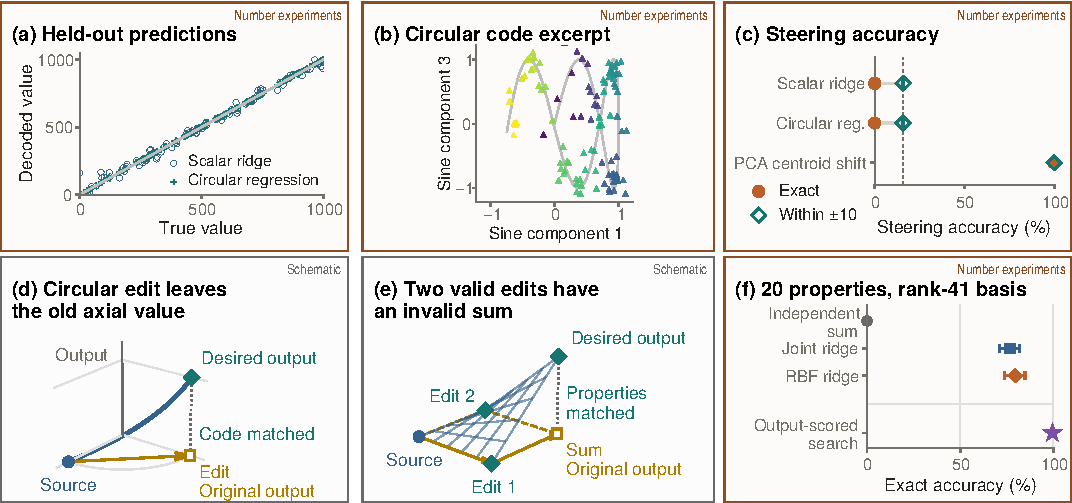
\includegraphics[width=\textwidth]{../figures/fig_numerical_sufficiency_atlas_space_optimized.pdf}
\caption{Probe-derived edits yield little control despite accurate numerical decoding.
(a,b) Scalar ridge and circular regression decode values and codes from 100 individual Llama-3.1-8B development prompts.
(c) On these prompts, edits from the same fits yield no exact target outputs (2,000 per method); a PCA centroid shift succeeds.
The dotted line gives no-edit accuracy within $\pm10$.
(d,e) Matching a circular code or summing valid property edits can preserve the source output.
(f) Joint predictors use source activations and patch displacements, with different doses from the independent sum (400 edits, 20 source prompts).
Output-scored search evaluates all 100 source prompts (2,000 edits).
Whiskers in (c,f) give 95\% source-prompt bootstrap intervals for fixed fits (Appendices~\ref{sec:numerical-probe-setup} and~\ref{sec:numerical-control-dimension}).}
\label{fig:numerical-sufficiency-atlas}
\end{figure*}
